% Forcing-probe section (RQ2), Xingjian Liu. DRAFT, 2026-11-12: MiMo-RL and Qwen-Instruct complete; MiMo-SFT without its RQ1 baseline; Qwen-Thinking all forcing runs and the 50-output hand check (no RQ1 baseline yet, so placement is compared with the user turn and with n=0 by analysis/place_tests.py; Homogeneous needs its Default run).
% Numbers marked \tbd wait for the other three models; MiMo-RL numbers are Unseen unless stated and
% come from results/mimo-rl-2508/ (data branch rq2/forcing-results) via analysis/forcing_table.py.
% Needs \usepackage{xcolor,booktabs,graphicx} and the proposal's references.bib.
\providecommand{\tbd}{\textcolor{red}{TBD}}

\section{Forcing probes: what the earlier labels do to B}
\label{sec:forcing}

RQ1 shows that B is named less often when all five objects are asked together than when it is asked
alone. The forcing probes ask whether that gap comes from the labels of the other four objects. They
replace the model's own earlier answers with labels we choose and measure what happens to B.

\paragraph{Probes.} All probes use the 502 Adversarial images in both orders (Seen 168, Unseen 334 per
order), the official multi-object prompt and greedy decoding. \emph{Incremental teacher forcing} is
ROPE's official procedure: five calls, where call $k$ states the true labels of objects $1,\dots,k-1$
and asks object $k$. In AAAAB, B is asked last, after four true A labels; in BAAAA it is asked first
with nothing given, so BAAAA is the order control. \emph{One-shot teacher forcing} makes a single call
that states the true labels of the four other objects and then asks B (in BAAAA it lists objects 2--5
and asks object 1 last), so the labels always come before the question in the text. The
\emph{counterfactual prefix} (CF) is the one-shot call with all four given labels replaced by one wrong
class C that is not in the image, drawn per image with a fixed seed. Four variants refine the one-shot
probe. \emph{Dose}: give only the first $n\in\{0,\dots,3\}$ of the four labels; $n=0$ keeps the
multi-object prompt and its \texttt{obj5:} cue, so comparing with $n=0$ isolates the labels.
\emph{Placement}: write the labels as the start of the model's own answer (after its reasoning)
instead of into the user turn. \emph{C near / far}: choose as C the remaining candidate whose name is
most or least similar to A (cosine of all-mpnet-base-v2 name embeddings; mean similarity to A is 0.49
for near, 0.27 for random and 0.13 for far). \emph{Homogeneous control}: one-shot teacher forcing on
Homogeneous items, where all five objects share a class and following the labels is correct.

\paragraph{Measures.} For each B we record whether it is named correctly, labelled A (inertia) or
labelled C. We follow the shared protocol: the tolerant parser is primary, a call that reaches the
token limit counts as wrong, every comparison is paired on the same images with an exact McNemar test
and a bootstrap 95\% CI, and $p$-values are Holm-adjusted over the comparisons of one model with the
same reference within one probe family (the core probes of Table~\ref{tab:forcing}, the dose series,
placement, C near / far, and the Homogeneous control). Because a cut call can never be A, we repeat each comparison on the images where
neither call was cut. For the dose series we also report the per-image least-squares slope of B=A over
$n$, with a permutation test that shuffles $n$ within each image.

\begin{table*}[t]
\centering\small
\begin{tabular}{l rr rr rr rr}
\toprule
& \multicolumn{2}{c}{MiMo-SFT} & \multicolumn{2}{c}{MiMo-RL} & \multicolumn{2}{c}{Qwen-Instruct} & \multicolumn{2}{c}{Qwen-Thinking} \\
Condition & AAAAB & BAAAA & AAAAB & BAAAA & AAAAB & BAAAA & AAAAB & BAAAA \\
\midrule
Single-object            & \tbd & \tbd & 18.9 & 24.0 & 20.1 & 22.8 & \tbd & \tbd \\
Default                  & \tbd & \tbd & 29.3 & 32.6 & 35.9 & 25.1 & \tbd & \tbd \\
TF incremental           & 51.2 & 32.9 & 40.7$^{*}$ & 33.2 & 41.0 & 25.4 & 42.2 & 32.0 \\
TF one-shot              & 51.5 & 34.4 & 42.5$^{*}$ & 35.3 & 41.3 & 32.6$^{*}$ & 41.6 & 36.2 \\
CF (B labelled A)        & 43.1 & 35.3 & 35.6$^{*}$ & 35.3 & 10.8$^{*}$ & 18.9$^{*}$ & 33.8 & 34.4 \\
CF (B labelled C)        & 1.8 & 0.6 & 0.3 & 0.6 & 41.0 & 21.0 & 0.9 & 1.8 \\
TF one-shot, in answer   & 49.1 & 40.1 & 32.6 & 36.8 & 47.6$^{*}$ & 44.9$^{*}$ & 44.9 & 34.1 \\
CF in answer (B labelled C) & 79.0 & 86.5 & 36.8 & 56.3 & 83.5 & 83.2 & 64.4 & 53.0 \\
\bottomrule
\end{tabular}
\caption{B labelled A (\%) on Unseen Adversarial items under each probe (tolerant parser; the two
``B labelled C'' rows give B labelled C instead). ``In answer'': the given labels are written as the
start of the model's answer; the label scored is the first one it writes for B. $^{*}$: differs from
Default, Holm-adjusted $p<0.05$ (exact McNemar, paired). MiMo-SFT and Qwen-Thinking have no Default or
Single-object run yet (RQ1, \tbd), so their rows carry no test. For MiMo-RL, B=A under Default and every forcing probe differs from Single-object at Holm
$p<0.01$. Seen, accuracy and strict scores:
Appendix~\tbd.}
\label{tab:forcing}
\end{table*}

\paragraph{Correct labels pull B toward A when B is box 5.} On MiMo-RL, stating the four true A labels
raises B=A on AAAAB from 29.3\% (Default) to 42.5\% (one-shot; $+13.2$ points, Holm $p<10^{-5}$) and
to 40.7\% (incremental; $+11.4$), against 18.9\% when B is asked alone (Table~\ref{tab:forcing}). The
rise holds on images where no call was cut ($+11.4$). Accuracy on B falls by 4.8 points, which is not
significant after correction. The effect grows with the number of labels given
(Figure~\ref{fig:dose}): B=A rises by 2.6 points per label (95\% CI 1.7--3.6, permutation $p<0.001$),
from 32.9\% with none to 42.5\% with all four; $n=0$ does not differ significantly from Default
($+3.6$). On Seen items (168 per order) the direction is the same (AAAAB: 20.8\% to 28.6\%, $+7.7$)
but not significant after correction, while the dose slope is ($+2.1$ points per label, Holm
$p=0.001$).
The pull is stronger in MiMo-SFT. Its dose slope on AAAAB is 5.0 points per label (Unseen; 5.1 on
Seen), about twice MiMo-RL's, and B=A reaches 51.5\% with all four labels. Whether RL training weakens
the pull or only moves the baseline needs MiMo-SFT's Default run (\tbd). Qwen-Instruct is pulled as
well: its dose slope on AAAAB is 2.7 points per label. So is Qwen-Thinking: 3.0 points per label
(95\% CI 2.0--4.0, Holm $p<0.001$), and all four labels raise its B=A from 29.9\% to 41.6\%
($+11.7$; $+10.7$ on images where neither call was cut).

\paragraph{When B is box 1, the same labels barely matter.} In BAAAA the one-shot prompt also lists
the four A labels before asking B, yet B=A rises only 2.7 points (not significant) and the dose slope
is 0.8 points per label (Holm $p=0.10$). The text order of labels and question is the same in both
orders, so the pull depends on where B sits among the boxes. The model's answers suggest why: in
99.7--100\% of answered rows it rewrites all five labels in box order rather than continuing from the
given ones, so in AAAAB it writes A four times just before B, and in BAAAA it writes B first.
A hand check of 50 raw outputs agrees. All 34 with labels in the user turn rewrite the whole list:
with fewer than four labels given the model labels the other boxes itself, in 6 of the 26 with true
labels it changes at least one of them, and under CF it always replaces C with its own classes.
MiMo-SFT answers the same way (all 34 rewrite the list), and so does Qwen-Thinking: it writes all
five labels in every answered row and never continues from the given ones (all 34 checked answers
rewrite the list; it changes a true label in 3 of 26). Qwen-Instruct does not. In 27 of 34 checked
answers it continues from the given labels and writes B right after them. It is also pulled in
BAAAA: one-shot teacher forcing raises B=A from 25.1\% to 32.6\% ($+7.5$, Holm $p<0.001$), and its
dose slope there is 1.6 points per label ($p<0.001$). For these three models, what matters is what
the model has just written before B, not where B sits in the prompt. Qwen-Thinking does not fit this
rule. It rewrites the list like the MiMo models, so B is the first label of its BAAAA answer, yet its
dose slope there is 1.5 points per label (95\% CI 0.7--2.3, Holm $p<0.001$), half its slope on AAAAB
and close to Qwen-Instruct's, and all four labels raise B=A by 5.7 points (CI 2.4--9.3; $+5.5$ on
images where neither call was cut). On Seen items its BAAAA slope is 2.3 points per label (Holm
$p<0.001$). Section~\ref{sec:discussion} returns to this.

\paragraph{The model rejects a wrong class but still drifts to A.} Under CF, MiMo-RL almost never
copies C: B is labelled C in 0.3--1.2\% of items, and C survives on any of the four given boxes in
under 2\% of answers. Instead the model relabels those boxes, mostly as A (64.1\% Unseen, 74.5\% Seen
of answers). B=A still rises on AAAAB ($+6.3$, Holm $p=0.04$). Here the A labels before B are the
model's own, which is the self-induced part of RQ2. CF also changes the question (B is asked after
four given labels), so this probe alone does not separate the two causes. MiMo-SFT behaves the same
way (B labelled C in 0--2.4\% of items), and so does Qwen-Thinking (0.9--1.8\%; C survives on a given
box in at most 2.5\% of answers, and 70--77\% relabel all four given boxes A). Qwen-Instruct does not: it copies C onto B in 41.0\% of
AAAAB and 21.0\% of BAAAA items, and B=A falls well below Default.

\paragraph{A wrong class close to A is accepted more, but B drifts the same.} Choosing C by its
similarity to A changes how often C is accepted. With the remaining class most similar to A as C,
C survives on a given box in 8.1\% (Unseen) and 21.8\% (Seen) of answers, and B is labelled C 1.8
and 3.9 points more often than with a random C (both orders; Holm $p=0.03$ and $0.07$). With the
least similar class, both stay at the level of a random C. B=A does not differ significantly between
near, random and far C. MiMo-SFT and Qwen-Thinking show the same pattern. Pooled over both orders,
near C is copied onto B more often than far C: by 3.9 and 3.3 points on Unseen (Holm $p<0.001$ for
both) and by 4.5 and 5.7 on Seen (Holm $p=0.02$ and $0.008$). Their B=A does not change either.
Qwen-Instruct, which copies C far more often, does not accept a near C more than a random one. The
drift of B toward A thus does not depend on how plausible the injected class is.

\paragraph{Following labels helps when they are right.} On Homogeneous items, the same one-shot probe
raises accuracy on box 5 from 80.4\% to 86.9\% ($+6.5$, Holm $p<10^{-3}$; Seen: 87.0\% to 96.0\%),
and Qwen-Instruct's from 85.3\% to 95.9\% ($+10.6$).
The labels are not ignored; the model leans on them whether or not the object matches.

\paragraph{Labels written as the model's own answer.} When the same four true labels are written as
the start of the model's answer, after its reasoning, MiMo-RL's first label for B on AAAAB is A in
32.6\% of items: close to Default ($+3.3$ points, not significant) and well below the 42.5\% for the
same labels in the user turn (BAAAA: 36.8\%, also not significant). The true labels thus pull B
toward A mainly through the reasoning that follows them, not by being copied in the answer line.
A wrong class behaves differently. After four forced C labels, the first label for B is C in 36.8\%
(AAAAB) and 56.3\% (BAAAA) of items (Seen: 31.5\% and 48.8\%), against at most 1.2\% when the same
labels are given in the user turn, and it is never A. Here the forced line contradicts the model's
own reasoning, and the answer still continues it. The model often notices: it keeps writing after
the label in 62--76\% of items, typically ``Wait, no, that's wrong'' and a re-check, and in
28--40\% it starts its own five-label list on a new line. By the end of the answer, B is C in 8.4\%
(AAAAB) and 26.0\% (BAAAA) of items. The answer text therefore carries an inertia of its own, which
the model's re-check only partly undoes. MiMo-SFT and Qwen-Instruct never re-check: each writes one
label after the forced line and stops. After four forced C labels, B is C in 79.0\% and 86.5\% of
items for MiMo-SFT and 83.5\% and 83.2\% for Qwen-Instruct (AAAAB and BAAAA). Qwen-Instruct has no
reasoning that could override the labels, so for it true labels in its own answer pull hardest: B=A
rises by 11.7 and 19.8 points over Default. Qwen-Thinking reasons but does not re-check either: it
keeps writing after the label in at most 0.3\% of items (none of 16 checked by hand), and after four
forced C labels B is C in 64.4\% (AAAAB) and 53.0\% (BAAAA) of items (Seen: 58.9\% and 44.6\%).
Unlike MiMo-RL, it follows true labels in its own answer as much as in the user turn: on AAAAB, B=A
is 44.9\% against 41.6\% (not significant) and 15.0 points above the one-shot prompt with no labels
(Holm $p<10^{-8}$; Qwen-Thinking has no Default run yet). Seen items agree: 30.4\% against 32.7\%,
and 9.5 points above no labels (Holm $p=0.002$). On BAAAA the labels in its answer add 3.6 points
over no labels (Seen: 4.8), which is not significant.

\begin{figure}[t]
\centering
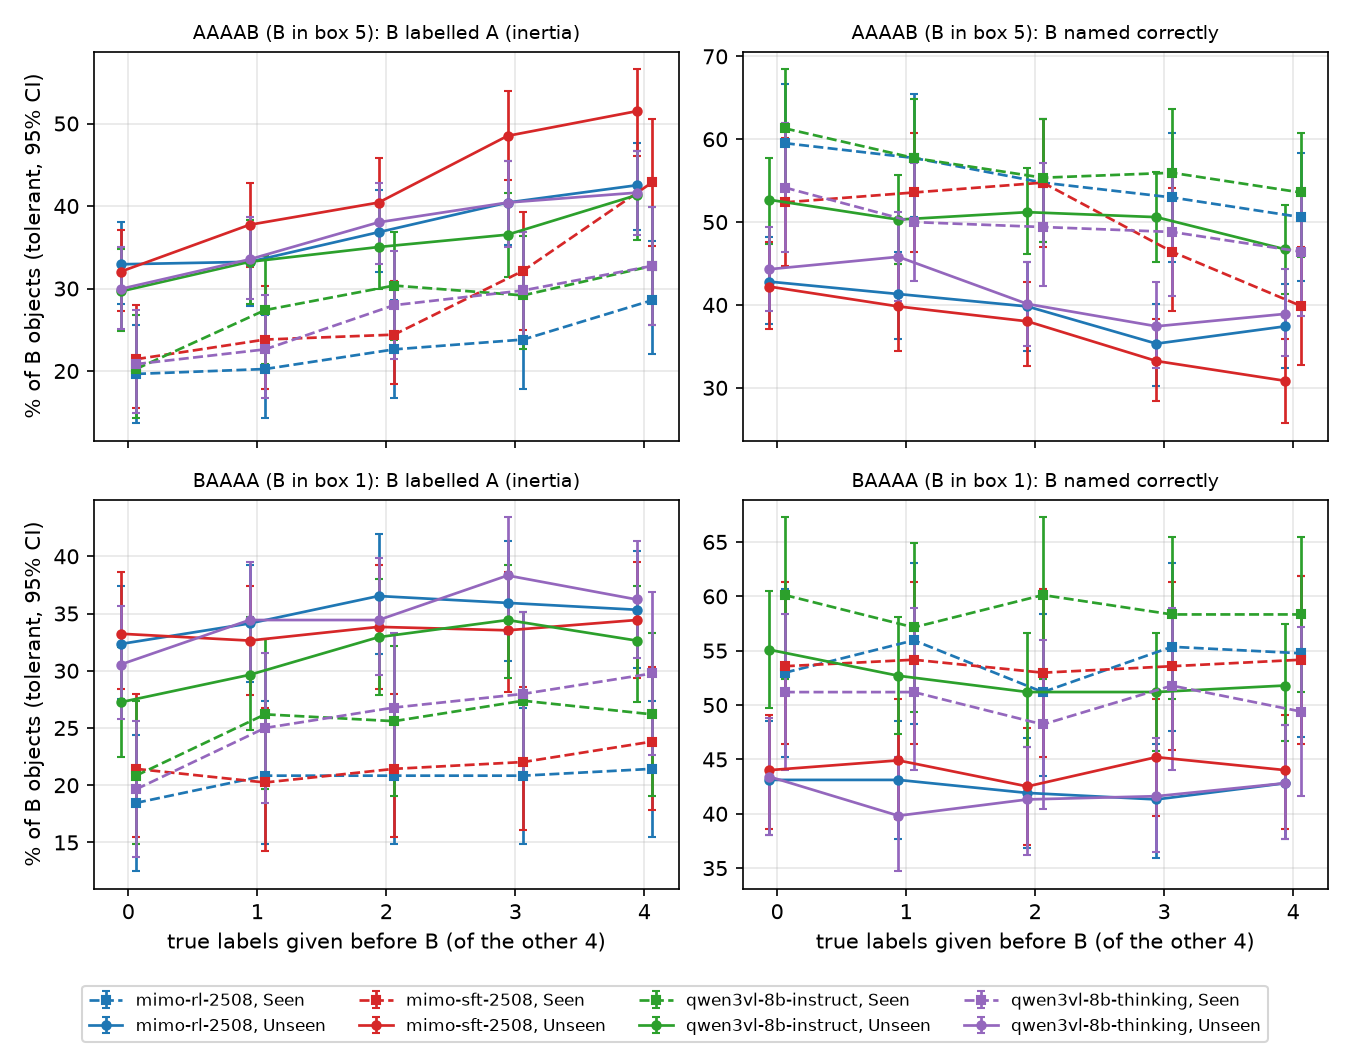
\includegraphics[width=\columnwidth]{figures/forcing_fig4_dose.png}
\caption{B labelled A and B named correctly against the number of true A labels given before B
(one-shot teacher forcing, all four models; 95\% bootstrap CIs). Solid: Unseen; dashed: Seen.
$n=4$ is the TF one-shot run. Drawn by \texttt{analysis/forcing\_table.py} from the dose and TF
one-shot files on the data branch.}
\label{fig:dose}
\end{figure}
